\section{Abstrakte Architektur}
In diesem Dokument soll ein Transportsystem mit autonom agierenden Transportvehikeln (\emph{Robots})
entwickelt werden, welche Notfalltransporte für ein Krankenhaus (\emph{Hospital}) erledigen. Die \emph{Robots} werden zu
einem vom \emph{Hospital} angegebenen Ort geschickt, um dort einen Patienten (\emph{Patient}) abzuholen und
danach zur Klinik zu fahren.

Dieser Entwurf basiert auf der in der Analyse erarbeiteten Spezifikation des Systems. Abbildung \ref{KomponentendiagrammAbstrakt} zeigt das abstrakte Komponentendiagramm.

\begin{figure}[H]
	\centering
	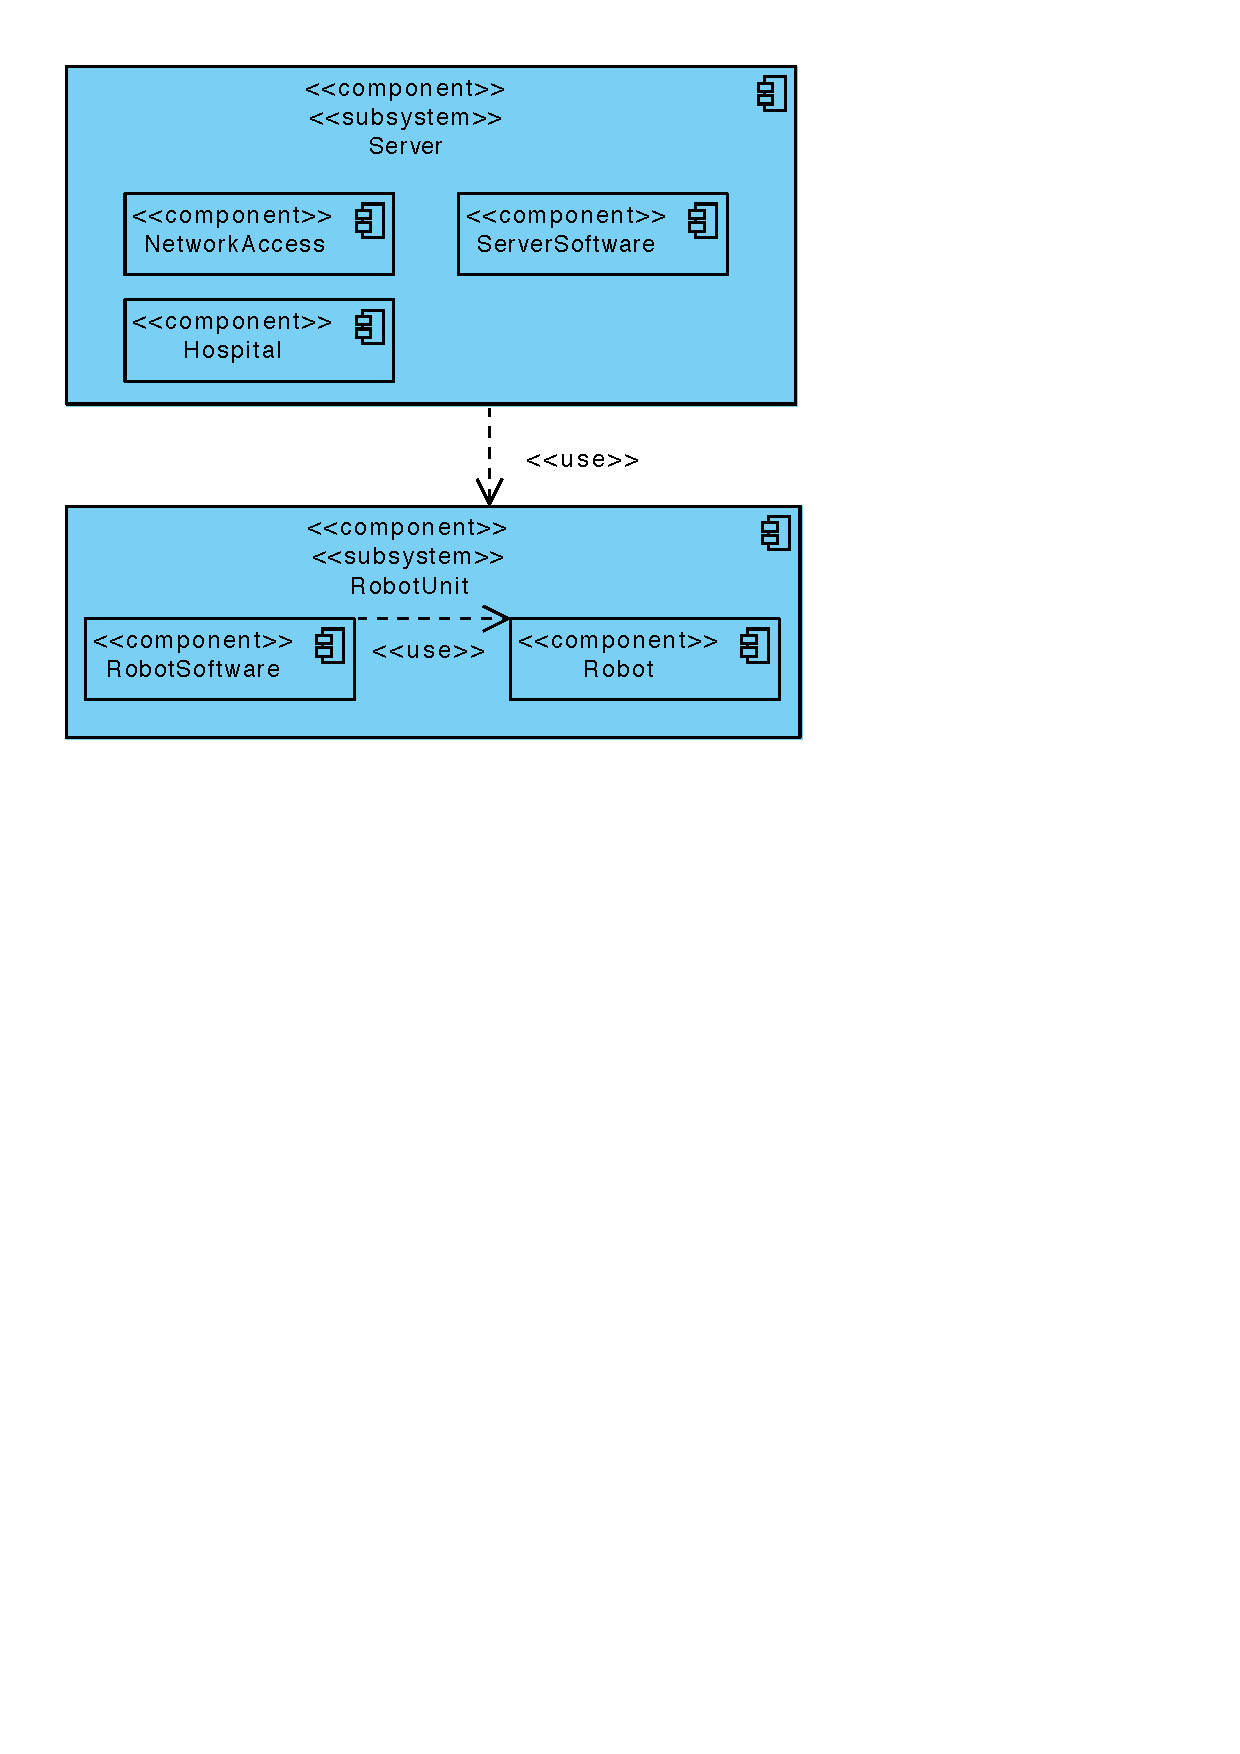
\includegraphics[width=0.6\textwidth]{img/AbstrakteArchitektur}
	\caption{Abstraktes Komponentendiagramm}
	\label{KomponentendiagrammAbstrakt}
\end{figure}

Da eine Komponente mit dem Namen \emph{Robot} bereits vorhanden ist, nennen wir die \emph{Robot}-Hauptkomponente \emph{RobotUnit}. Dieser Name verdeutlicht, dass jeder physische Roboter im System durch diese Hauptkomponente repr\"{a}sentiert wird.


In diesem Kapitel wird die im Rahmen der Analyse ermittelte Einteilung des Systems in Komponenten strukturiert dargestellt. Hierbei soll auch die Interaktion der Komponenten untereinander verdeutlicht werden.

\subsection{Server}

Der \emph{Server} verwaltet die \emph{Tasks} f\"{u}r die \emph{RobotUnits} und beh\"{a}lt einen st\"{a}ndigen \"{U}berblick \"{u}ber die Positionen der \emph{RobotUnits}. Er ist f\"{u}r die effiziente Allokation der Auftr\"{a}ge f\"{u}r die \emph{RobotUnits} zust\"{a}ndig.

\subsubsection{NetworkAccess}

Die Komponente \emph{NetworkAccess} dient der Kommunikation mit dem Netzwerk.

\subsubsection{Hospital}

Die Komponente \emph{Hospital} dient der Kommunikation mit dem Krankenhaus.

\subsubsection{ServerSoftware}

Die Komponente \emph{ServerSoftware} ist die Verwaltungslogik des \emph{Servers}. Sie greift auf die serverseitigen Subsysteme zu und stellt die zentrale Anlaufstelle f\"{u}r alle \emph{RobotUnits} dar. 

Bei einer Anfrage ermittelt sie die passende \emph{RobotUnit} und sendet ihr die Position des Ziels. 

\subsection{RobotUnit}

Die Komponente \emph{RobotUnit} sublimiert die \emph{RobotSoftware} und \emph{-Hardware} (Komponente \emph{Robot}) als eine Oberkomponente. Sie vereint alle Hard- und Softwareinterfaces dieser Komponenten und leitet die ein- und ausgehenden Nachrichten der \emph{RobotSoftware} an den \emph{Server} weiter. Sie dient somit als \"{u}bergeordnete Schnittstelle f\"{u}r die Kommunikation. 

\subsubsection{RobotSoftware}

Die \emph{RobotSoftware} steuert den \emph{Robot} an und verwertet seine Sensordaten. Dazu geh\"{o}rt unter anderem die Fahrlogik und die Verwaltung der \emph{Battery}, damit angenommene \emph{Tasks} auch komplett ausgef\"{u}hrt werden k\"{o}nnen und die \emph{RobotUnit} rechtzeitig die \emph{ChargingStation} erreicht. 

\subsubsection{Robot}

Die Komponente \emph{Robot} steht f\"{u}r alle hardwaretechnischen Spezifikationen des \emph{Robots}. Dazu geh\"{o}ren die Fahreinheit und die interne Sensorik sowie die \emph{Battery}.   